\chapter*{Struttura del software}

\section*{Linguaggi e framework}
L'applicazione ha come \textit{target platform} Android percio' il linguaggio usato principalmente e' stato Java. Da notare che su Android e' presente nella versione 7, percio' non sono disponibili alcune funzionalita' come i metodi di default, \textit{stream}, \textit{lambda expression} ecc.  Per rimediare soprattutto alla mancanza di quest'ultime, che migliorano la lettura e scrittura di alcune parti di codice, ho affiancato un altro linguaggio a Java: Kotlin. Senza fare un confronto tra i due linguaggi, Kotlin mi ha permesso di scrivere lambda expression compilando un bytecode perfettamente compatibile con Java 6.

\section*{Interfaccia grafica}
L'interfaccia e' stata realizzata ai fini di test pratici delle funzionalita' finali dell'applicazione quindi non ha una grande cura da un punto di vista estetico come vedremo piu' avanti.
La parte alta contiene delle label raffiguranti i 3 valori catturati tramite il magnetometro e presi tramite le API di Android. \\
Nel mezzo ci sono dei pulsanti per:
\begin{itemize}
	\item Iniziare/Terminare la scansione dell'ambiente.
	\item Incrementare la \textit{label} che verra' assegnata alla prossima \textit{fingerprint} registrata
	\item Iniziare/Terminare la ricerca.
	\item Serializzare tutti i dati registrati finora
	\item De-serializzare i dati salvati in un JSON.
\end{itemize}
Nella parte bassa invece c'e' una \textit{textbox} contenente il log che verra' stampato durante l'esecuzione del programma.

\begin{figure}[H]
\centering
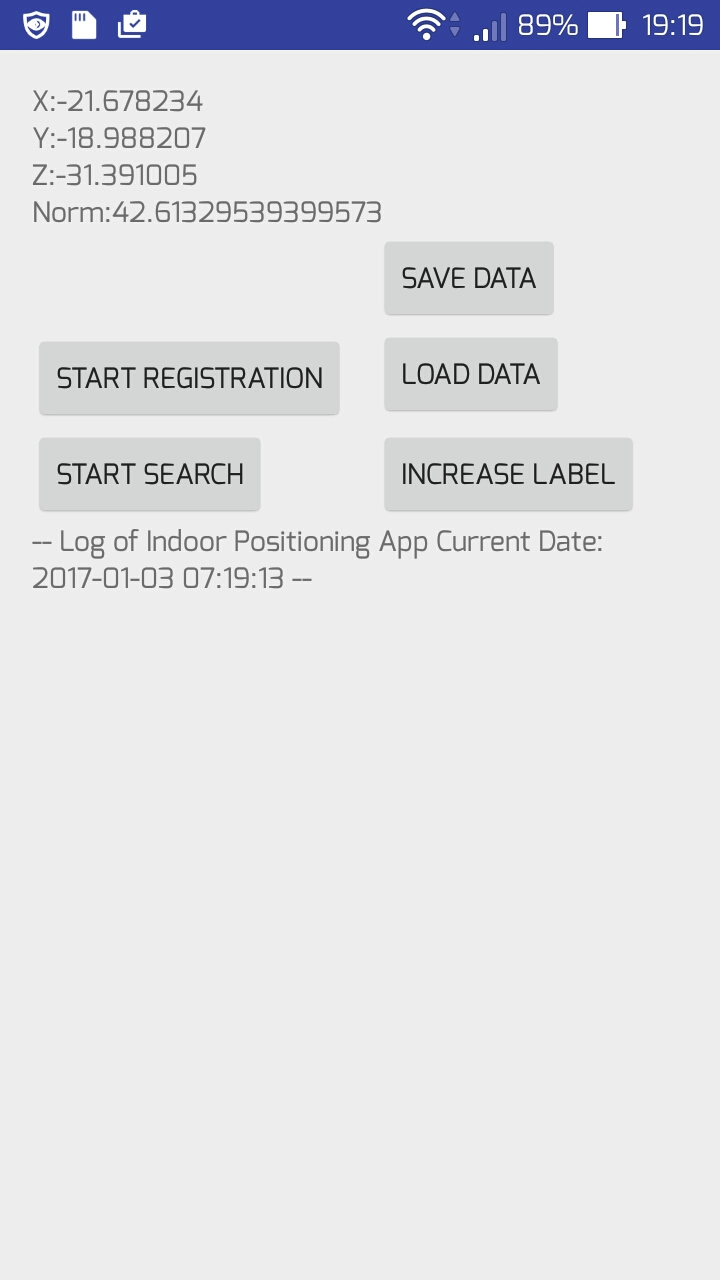
\includegraphics[width=0.3\linewidth]{img/app_screen}
\caption{Interfaccia grafica all'avvio dell'applicazione}
\label{fig:app_screen}
\end{figure}

\section*{Persistenza dei dati}
L'applicazione consente anche di serializzare tutti i dati registrati fino a quel momento nel formato standard JSON tramite la libreria \textit{gson} che fornisce delle funzioni  per il linguaggio Java per la serializzazione/de-serializzazione di oggetti. Il file viene salvato nella cartella dati dell'applicazione non visibile all'utente.

\section*{Struttura del codice e design pattern}
Nello sviluppo del software sono stati applicati vari \textit{design pattern} visti durante i vari corsi e principi di programmazione. Fra questi ultimi abbiamo il \textit{dependency inversion principle}, il \textit{open closed principle}. Riguardo i \textit{design pattern}, ho usato molto l'\textit{observer}, il \textit{template} e \textit{factory}.

\section*{Analisi dei dati}
La predizione dei risultati e' stata implementata sia nel software \textit{Android} sia sul computer. Nel codice mobile e' stato adoperato solamente il KNN per via della facilita' d'implementazione da zero e non e' stato  utilizzato per testare la precisione, ma per verificare il corretto funzionamento dell'applicazione. Invece su computer, presi i dati serializzati dal software mobile, sono stati applicati tutti gli algoritmi di apprendimento elencati precedentemente e gia' tutti implementati da librerie di terze parti per verificare la precisione dei dati. Il linguaggio scelto su computer e' \textit{Python} per via del suo buon supporto all' apprendimento automatico.